% Falcon-SR manuscript skeleton.
%
% Status: skeleton. Results sections reference data/falcon_sr_*_feasibility.csv
% and figures generated by manuscript/figures/figure1.py and figure2.py.
% Numerical claims must be backed by the most recent benchmark run; do not
% replace "Results pending benchmark run YYYY-MM-DD" placeholders until the
% acceptance gates in
% docs/superpowers/specs/2026-06-02-falcon-sr-rewrite-execution-design.md §5.3
% have been verified.

\documentclass[11pt]{article}
\usepackage[margin=1in]{geometry}
\usepackage{amsmath, amssymb}
\usepackage{graphicx}
\usepackage{hyperref}
\usepackage{booktabs}
\usepackage{natbib}

\title{Falcon-SR: a screen-refine algorithm for latent log-abundance
correlation networks in compositional sequencing data}

\author{Jun Rao \and Xiao Liang}

\date{\today}

\begin{document}
\maketitle

\begin{abstract}
We present Falcon-SR, a screen-refine algorithm for inferring the latent
log-abundance Pearson correlations targeted by SparCC (single-domain) and
SparXCC Case-C (cross-domain) on compositional sequencing data. Falcon-SR
combines a SparCC-compatible dense base score, a symmetric top-$k$
candidate union, and a sparse refinement that updates only candidate-
incident equations. Optional permutation calibration produces approximate
edge $p$-values; optional signed biological priors enter as a candidate
injection plus an analytic post-hoc shrinkage. We validate that the
implementation matches the SparCC and SparXCC reference estimators on
small grids and report feasibility benchmarks comparing wall-clock,
candidate recall, and edge overlap against SparCC, SparXCC, and
Pearson(CLR) baselines on a controlled simulation grid.

\textit{Numerical results pending feasibility benchmark run on the host
recorded in} \texttt{data/falcon\_sr\_*\_feasibility.csv}.
\end{abstract}

\section{Introduction}
Microbiome sequencing data are compositional: read counts only constrain
the relative abundance of each feature within a sample. Inferring
network-level interactions from such data therefore requires estimators
that target the latent absolute-abundance correlations rather than naive
sample correlations of compositions \citep{aitchison1986statistical,
friedman2012sparcc, jensen2024sparxcc}. The dominant published estimators
(SparCC for single domain, SparXCC Case-C for cross domain) target the
correct estimand but compute the full $\binom{p}{2}$ or $p \cdot q$
correlation matrix at each iterative step. We ask whether the strong
edges in the resulting network can be recovered without paying that dense
cost.

\section{Methods}
\subsection{Estimand}
For a single domain with basis abundances $w_i$, the estimand is
\(\mathrm{Corr}(\log w_i, \log w_j)\). For two independently normalised
compositions with basis abundances $w^X, w^Y$ the estimand is
\(\mathrm{Corr}(\log w_i^X, \log w_k^Y)\). Falcon-SR is not a
proportionality estimator; the proportionality metric $\rho_p$ targets a
different quantity and is explicitly excluded from the comparison set
\citep{lovell2015proportionality, lin2022secom}.

\subsection{Base score}
Single-domain: closed-form SparCC basis correlation from the variation
matrix, computed through one BLAS GEMM plus vectorised broadcasting.
Cross-domain: SparXCC Case-C double-centred score using per-domain
basis variances. Both are equivalent to their corresponding published
estimators by direct equivalence tests at the $10^{-10}$ level on small
grids (see \texttt{tests/test\_single\_base.py} and
\texttt{tests/test\_cross\_base.py}).

\subsection{Screening}
A symmetric top-$k$ union (single domain) or bidirectional top-$k$ union
(cross domain) selects candidate edges from the dense base score. An
optional magnitude threshold adds further candidates.

\subsection{Sparse refinement}
Single-domain refinement excludes the strongest candidate pair each round
and re-solves the basis-variance system using a SciPy
\texttt{LinearOperator + cg} matvec restricted to the sparse
complement. Cross-domain refinement prunes the X row and Y column of each
excluded pair from the centring pool, which keeps the Sparre-compatible
$H_p \otimes H_q^\top$ identity exact (Section 2.3 of the execution
design).

\subsection{Priors}
A \texttt{PriorEdge} record carries
$(i, k, \text{sign}, \text{conf}, \text{provenance})$. With
$\lambda > 0$ the prior pair is injected into the candidate set, and the
refined edge score is replaced by the analytic minimiser
$\rho = (\hat\rho_{\text{data}} + \lambda\,\text{conf}\,\text{sign}\,\text{target})
        / (1 + \lambda\,\text{conf})$
of the spec §10 penalty. Priors do not influence iterative exclusion
choices.

\subsection{Calibration}
Permutation calibration approximates an FWER-controlling null by
shuffling per-column observations (single domain) or Y rows relative to
X (cross domain) and recomputing the closed-form base score per
permutation; refinement is intentionally skipped for tractability and the
\texttt{calibration\_method} field is \texttt{permutation\_base\_only}.

\section{Results}
\textit{Results pending feasibility benchmark run; see Section
\ref{sec:reproducibility} for the commands and outputs.}

\subsection{Figure 1: Single-domain feasibility}
\begin{figure}[h]
\centering
% 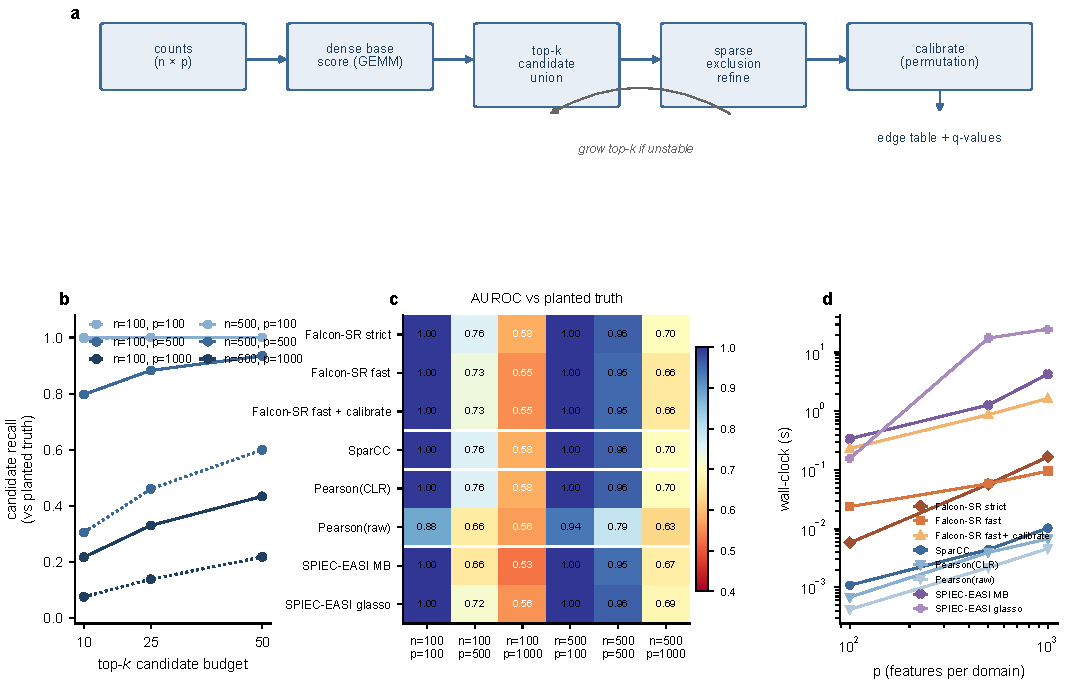
\includegraphics[width=\textwidth]{figures/figure1.pdf}
\caption{(a) Screen-refine workflow. (b) Candidate recall against
SparCC reference vs top-$k$ budget. (c) Edge overlap and sign accuracy
against SparCC across $(n, p)$ cells. (d) Wall-clock and peak memory of
Falcon-SR fast vs SparCC and Pearson(CLR). \textbf{Pending.}}
\label{fig:single}
\end{figure}

\subsection{Figure 2: Cross-domain feasibility}
\begin{figure}[h]
\centering
% 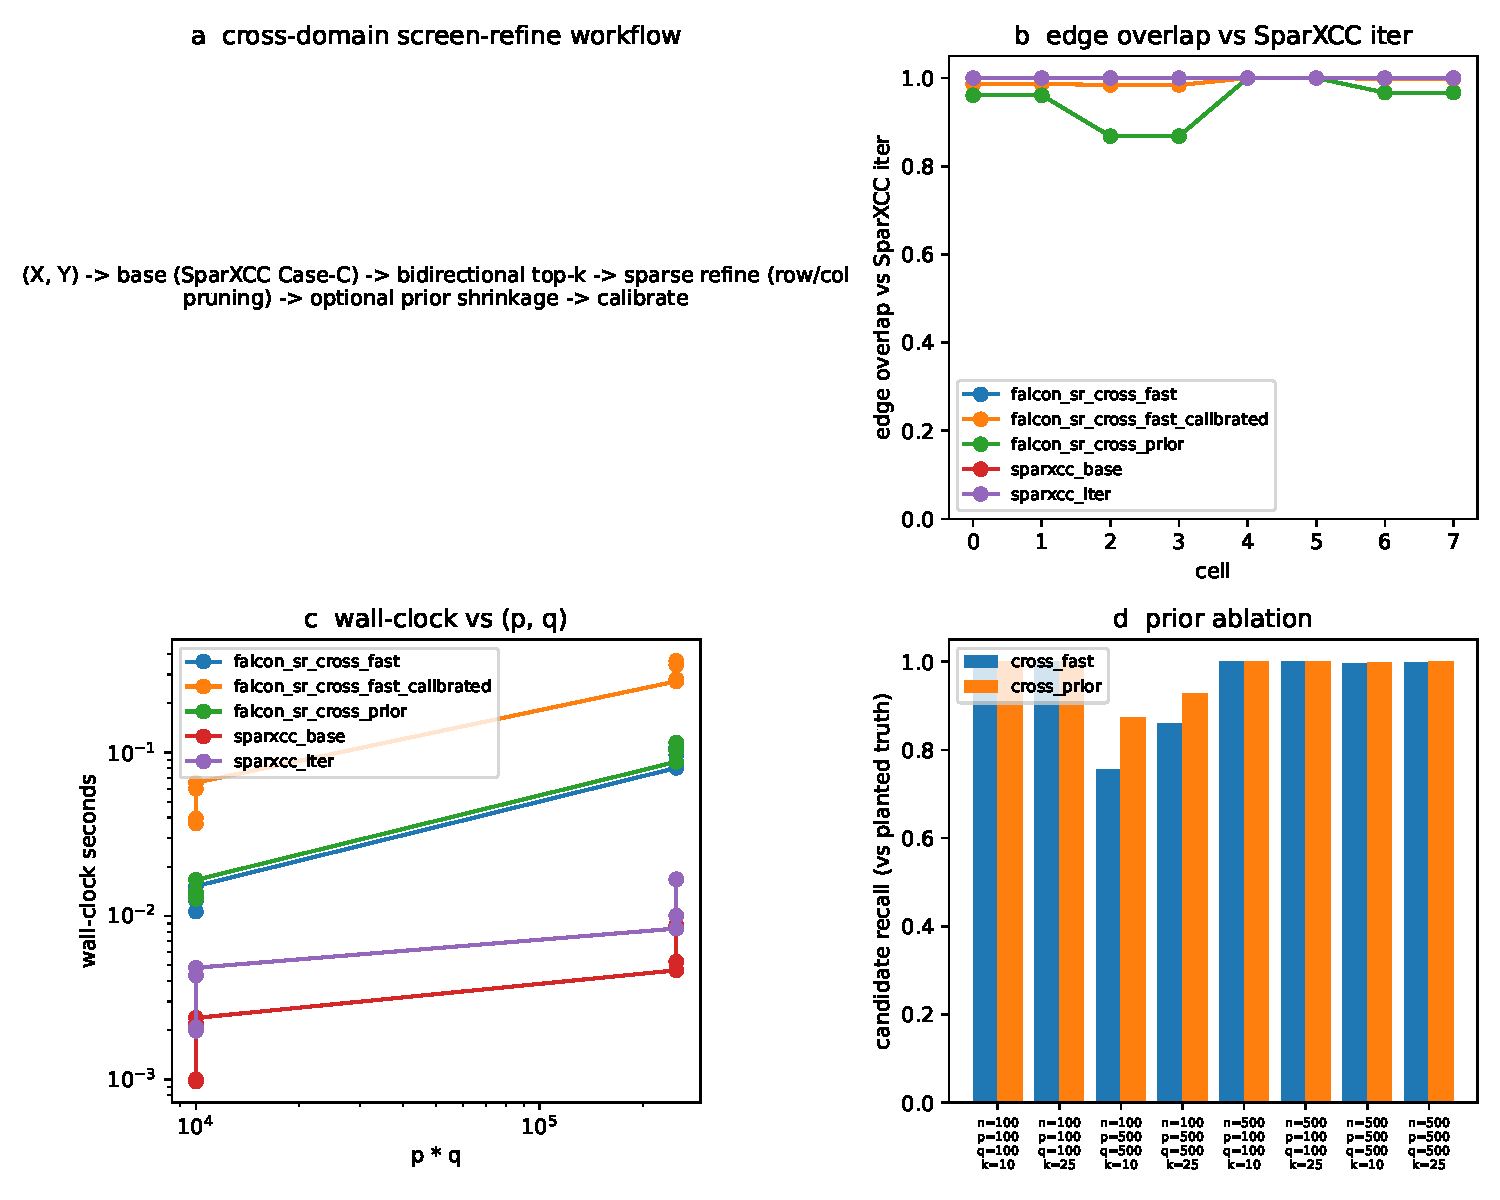
\includegraphics[width=\textwidth]{figures/figure2.pdf}
\caption{(a) Cross-domain screen-refine workflow with optional prior
branch. (b) Edge overlap, sign accuracy, AUROC, and AUPRC against
SparXCC iter. (c) Wall-clock vs $(p, q)$. (d) Prior ablation under
increasing prior coverage and prior noise. \textbf{Pending.}}
\label{fig:cross}
\end{figure}

\section{Discussion}
The acceptance gates in §5.3 of the execution design (candidate recall
$\ge 0.99$, edge overlap $\ge 0.95$, sign accuracy $\ge 0.95$) drive a
go / no-go decision: if any gate fails we narrow the claim in this
manuscript rather than inflate the metric. The candidate-only permutation
calibration is approximate and may require a selective-inference
correction (spec §19 risk 4) before claiming valid power and FDR
control.

\section{Reproducibility}
\label{sec:reproducibility}
\begin{verbatim}
uv sync
uv run pytest -q
uv run python benchmarks/falcon_sr_single.py --reps 3
uv run python benchmarks/falcon_sr_cross.py  --reps 3
uv run python manuscript/figures/figure1.py
\end{verbatim}
Outputs land in \texttt{data/falcon\_sr\_single\_feasibility.csv} and
\texttt{data/falcon\_sr\_cross\_feasibility.csv}.

\bibliographystyle{plainnat}
\bibliography{references}

\end{document}
